\renewcommand{\EntradaBibtex}{JaguarAplicacionMovil_2020}
\begin{frame}{\citetitle{\EntradaBibtex} \footnotemark[1] (1)}


%\begin{frame}{Desarrollos Tecnológicos}
\begin{block}{-} 
\begin{columns}
\begin{column}{0.48\textwidth}
		\begin{itemize}
		\item Detección de Codigos QR
		\item Modelado de la mascota en 3D mediante el Software Blender
		\item Sobreposición del modelo 3D dependiendo de la posición del código QR
		\end{itemize}
	\end{column}
	\begin{column}{0.52\textwidth}  
	    \begin{center}
	    	 
\includegraphics[width=0.25\textwidth]{Figs/JaguarFisico01}
	    	 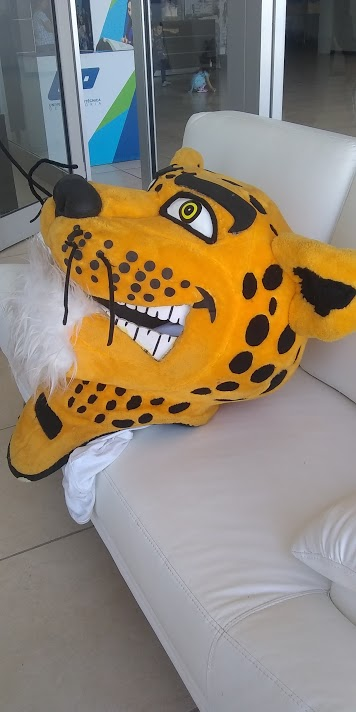
\includegraphics[width=0.25\textwidth]{Figs/JaguarFisico02}\\
    	 \end{center}
	\end{column}
	\end{columns}
	\end{block} 
	%\footnotetext{\fullcite{JaguarAplicacionMovil_2020}}
\footnotetext[1]{\fullcite{\EntradaBibtex}}
%\footnotetext{Andrés García González, Cristian Aléxis Lazo García, Damaris Mendoza Vázquez.  \textbf{Modelo 3D del Jaguar de la UPV sobre un código QR}. Universidad Politécnica de Victoria,  Informe técnico proyecto de asignatura ``Graficación por Computadora Aavanzada'', 2020. Sin Publicar.}
%\\setcounter{footnote}{0}
\end{frame}


\begin{frame}{\citetitle{\EntradaBibtex} (2)}
\begin{block}{-} 
\begin{columns}
	\begin{column}{0.98\textwidth}
	    \begin{center}
	    	 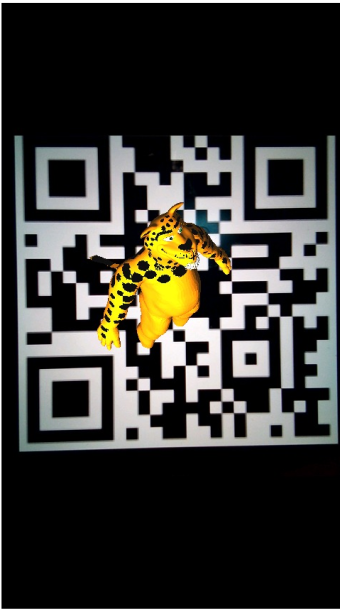
\includegraphics[width=0.24\textwidth]{Figs/JaguarVirtual01}
	    	 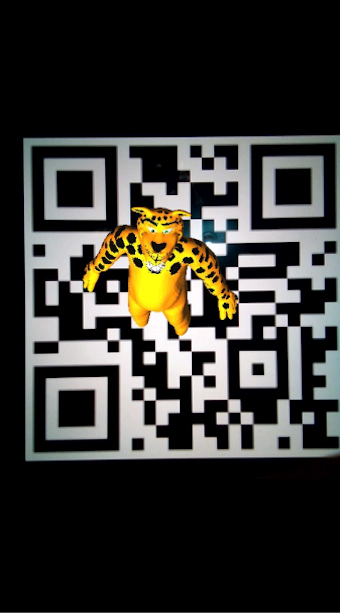
\includegraphics[width=0.24\textwidth]{Figs/JaguarVirtual02}
	    	 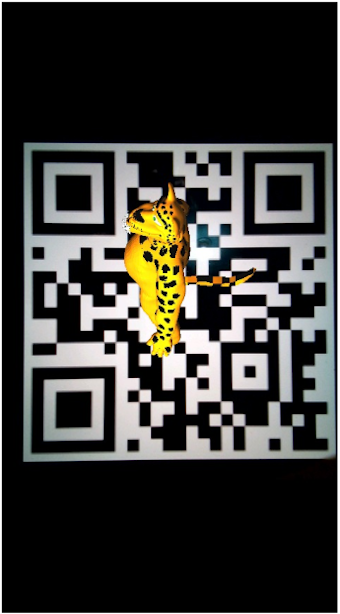
\includegraphics[width=0.24\textwidth]{Figs/JaguarVirtual03}
	    	 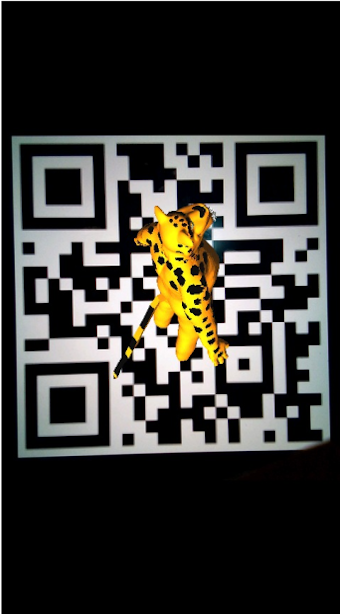
\includegraphics[width=0.24\textwidth]{Figs/JaguarVirtual04}
    	 \end{center}
	\end{column}
	\end{columns}
	\end{block} 
\end{frame}

